This approach has been tested initially on a linear feedback system of the form of $\bbsys$, interconnected to a linear exosystem $\bbexo$ \cite{galeani_optimal_2023}. Consider a continuous-time, linear time-invariant dynamic plant $\plant$ of the form
\begin{subequations}
	\label{eq:linplant}
	\begin{align}
		\dot{\plantstate}(t) & = \plantdynmat\plantstate(t) + \plantctrmat\plantinput(t), & t\in\R_{\geq 0}, \\
		\plantoutput(t)      & = \plantoutmat\plantstate(t), & t\in\R_{\geq 0},
	\end{align}
\end{subequations}
where $\plantstate(t)\in\R^\plantstatedim$ is the plant state vector, $\plantinput(t)\in\R^\plantinputdim$ is the control input, $\plantoutput(t)\in\R^\plantoutputdim$ is the plant output vector at time $t$, and $\plantdynmat\in\R^{\plantstatedim \times \plantstatedim}$, $\plantctrmat\in\R^{\plantstatedim \times \plantinputdim}$, and $\plantoutmat\in\R^{\plantoutputdim \times \plantstatedim}$ are constant matrices. In the considered setting, system \eqref{eq:linplant} is subject to a continuous-time, linear time-invariant feedback controller $\ctrl$ given by
\begin{subequations}
	\label{eq:lincontroller}
	\begin{align}
		\dot{\ctrlstate}(t) & = \ctrldynmat\ctrlstate(t) + \ctrlctrmat\plantoutput(t) + \ctrlrefmat\bbref(t), & t\in\R_{\geq 0}, \\
		\ctrlouput(t)       & = \ctrloutmat\ctrlstate(t), & t\in\R_{\geq 0},
	\end{align}
\end{subequations}
where $\ctrlstate(t)\in\R^{\ctrlstatedim}$ is the controller state vector and $\ctrlouput(t)\in\R^\ctrloutputdim$ is the controller output vector at time $t$, and $\ctrldynmat\in\R^{\ctrlstatedim\times\ctrlstatedim}$, $\ctrlctrmat\in\R^{\ctrlstatedim\times\bboutodim}$, $\ctrlrefmat\in\R^{\ctrlstatedim\times\bbrefdim}$, and $\ctrloutmat\in\R^{\ctrloutputdim\times\ctrlstatedim}$ are constant matrices. The interconnection of the plant $\plant$ and the control system $\ctrl\;$ forms the feedback loop $\bbsys$ according to $\plantinput = \ctrlouput + \bbaux$, with the dimension of the full state vector being $\bbstatedim = \plantstatedim + \ctrlstatedim$; to keep the notation as concise as possible, the plant output $\plantoutput$ is considered as the regulated output of the system $\bbsys$, \emph{i.e.}, $\bbouto = \plantoutput$, unless specified otherwise. The following assumption characterizes the properties of the feedback interconnection.
\begin{assumption}
  \label{ass:lqrall_closedloop}
  The pairs $(\plantdynmat,\plantctrmat)$, $(\ctrldynmat,\ctrlctrmat)$ are reachable, and the pairs $(\plantoutmat,\plantdynmat)$, $(\ctrloutmat,\ctrldynmat)$ are detectable. Moreover, the closed-loop feedback interconnection of \eqref{eq:linplant} and \eqref{eq:lincontroller} does not induce pole-zero cancellations and it is asymptotically stable.\closestatement
\end{assumption}

Let $s$ be a variable taking values in $\C$, and $\planttf(s)$ be the transfer matrix of system \eqref{eq:linplant} from $\plantinput$ to $\plantoutput$, computed from the state-space description of $\plant$. Let $\plantalltf(s)$ be the transfer matrix of \eqref{eq:bbsys} from $\bbaux$ to $\plantoutput$; moreover, let $(\bbdynmat,\bbctrmat,\bboutmat,0)$ be a realization of $\plantalltf(s)$. The Smith-McMillan degrees of $\planttf(s)$ and $\plantalltf(s)$ coincide with those of their respective state-space description thanks to \Cref{ass:lqrall_closedloop}.

The reference input in this setting is defined as the state of the exosystem $\bbexo$, which is a continuous-time linear time-invariant system of the form
\begin{subequations}
	\label{eq:linexosystem}
	\begin{align}
		\dot{\bbexostate}(t) & = \exodynmat\bbexostate(t), & t\in\R_{\geq 0}, \\
		\bbref(t)            & = \bbexostate(t), & t\in\R_{\geq 0},
	\end{align}
\end{subequations}
where $\bbexostate(t)\in\R^{\bbexostatedim}$ is the state vector at time $t$ and $\exodynmat\in\R^{\bbexostatedim \times \bbexostatedim}$ is a block-diagonal matrix defined as
\begin{subequations}
	\label{eq:linexoblocks}
	\begin{align}
    \exodynmat & = \diag(\exodynmat_0,\dotsc,\exodynmat_h), \\
		\exodynmat_0 & = 0,	\exodynmat_i = \begin{bmatrix} 0 & \omega_i \\ -\omega_i & 0 \end{bmatrix}, &  & i=1,\dotsc,h,
	\end{align}
\end{subequations}
with $\bbexostate(0) = \bbexostate_0\in\R^{\bbexostatedim}$. The angular frequencies $\{\omega_1,\dotsc,\omega_h\}$ in \eqref{eq:linexoblocks} are positive integer multiples of $2\pi/\bbperiod$, \emph{i.e.}, such that $\omega_i = k_i\frac{2\pi}{\bbperiod}$, $k_i\in\N$, $i=1,\dotsc,h$.

The feedback controller \eqref{eq:lincontroller}, together with exosystem \eqref{eq:linexoblocks}, ensure that \Cref{ass:bbiss,ass:bbssresp} hold. The complete block diagram of the closed loop is shown in \Cref{fig:lqrall}.
\begin{figure}[t!]
  \centering
  \includesvg[width=.9\linewidth]{images/ch7/lqrall/lqrall.svg}
  \caption{Block diagram of the feedback control system \eqref{eq:linplant}--\eqref{eq:lincontroller} interconnected to the exosystem \eqref{eq:linexosystem}; the input allocation device is enclosed in the $\mathcal{A}\ell\ell$ block.}
  \label{fig:lqrall}
\end{figure}

Both the transfer matrices $\planttf(s)$ and $\plantalltf(s)$ admit left coprime polynomial factorizations (see \cite[§7.8]{chen_linear_2009}) of the form
\begin{subequations}
	\label{eq:lqrall_lcfs}
	\begin{align}
		\planttf(s)      & = \plantlcfd^{-1}(s)\plantlcfn(s)\label{eq:lqrall_plantlcf}, \\
		\plantalltf(s)   & = \plantalllcfd^{-1}(s)\plantalllcfn(s)\label{eq:lqrall_looplcf},
	\end{align}
\end{subequations}
where $\plantlcfd(s)$, $\plantalllcfd(s)$, $\plantlcfn(s)$ and $\plantalllcfn(s)$ are polynomial matrices. The following assumption is introduced to simplify the discussion.
\begin{assumption}
  \label{ass:lqrall_kernels}
  The left coprime factorization \eqref{eq:lqrall_lcfs} is such that the following holds:
	\begin{subequations}
		\label{eq:lqrall_kernels}
		\begin{align}
			 \ker(\plantalllcfn(0)) &= \ker(\plantlcfn(0)),                                   \\
			 \ker(\plantalllcfn(j\omega_i)) &= \ker(\plantlcfn(j\omega_i)), &  & i=1,\dotsc,h.
		\end{align}
	\end{subequations}
	\closestatement
\end{assumption}

Although the factorization \eqref{eq:lqrall_lcfs} is not unique, it can be shown that \Cref{ass:lqrall_kernels} holds for one of them if and only if it holds for each one of them. The performance output in this case is defined as the plant input, \emph{i.e.}, $\bboutp = \plantinput$. The effort demanded to the actuators is thus evaluated by the instantaneous cost function $\ell(\bbssoutp(t)) = \left\Vert \plantssinput(t) \right\Vert^2_2$. Setting $\tau_0=0$ in eq.~\eqref{eq:bbcost} yields the following formulation of the cost functional $J$:
\begin{equation}
  \label{eq:lqrall_sscost}
  J(\plantssinput) = \frac{1}{2} \int_{0}^{T} \left\Vert \plantssinput(\tau) \right\Vert^2_2\,d\tau.
\end{equation}

Requirements (P), (I), and (O) of \Cref{prb:ssinv} reveal the connection between \emph{dynamic control allocation} on one hand and \emph{constrained optimal control} on the other: the (P) statement requires the asymptotic behavior to be $\bbperiod$-periodic, the (O) statement introduces the cost to optimize, and finally the (I) statement describes the constraint to be satisfied to ensure that the optimal steady-state solution does not affect the original steady-state output performance induced by the controller \eqref{eq:lincontroller}. To substantiate this evidence, the definition of a few more items is required. Let $(\feedbackdynmat,\feedbackctrmat,\feedbackoutmat,0)$ be a minimal state-space realization of the feedback loop $\bbsys$ having $\bbexostate$ as input and $\ctrlouput$ as output. Let $\Pi\in\R^{\bbstatedim \times \bbexostatedim}$ be the solution of the Sylvester equation
\begin{subequations}
	\label{eq:lqrall_memontinv_mbar}
	\begin{equation}
		\label{eq:lqrall_memontinv}
		\Pi \exodynmat = \feedbackdynmat\Pi + \feedbackctrmat,
	\end{equation}
	and define $\bar{M}\in\R^{\bbauxdim \times \bbexostatedim}$ as
	\begin{equation}
		\label{eq:lqrall_mbar}
		\bar{M} = \feedbackoutmat\Pi,
	\end{equation}
\end{subequations}
which is termed the \emph{pseudo-steady-state output map}. Let $\ctrlssoutput$ denote the steady-state controller output. The following equality holds (see \Cref{app:moments}, as well as \cite{astolfi_model_2010,scarciotti_data-driven_2017} for a proof):
\begin{align}
  \label{eq:lqrall_ssctrl}
	\ctrlssoutput(t) &= \bar{M}\bbexostate(t), & t\in\R_{\geq 0}.
\end{align}
The finite-horizon optimal control problem corresponding to \Cref{prb:ssinv} is formulated as follows.

\begin{problem}[Optimal input allocation for linear dynamics]
	\label{prb:lqrall_optcont}
	Consider the continuous-time, linear time-invariant feedback control system described by \eqref{eq:linplant}, \eqref{eq:lincontroller}, and the exosystem \eqref{eq:linexosystem}. Suppose that \Cref{ass:bbiss,ass:bboveract,ass:bbssresp,ass:lqrall_closedloop,ass:lqrall_kernels} hold, and define $\bar{M}$ as in \eqref{eq:lqrall_memontinv_mbar}.
	Determine, if it exists, a function $v^{\star}\in\mathcal{L}_2([0,\bbperiod])$ that
	\begin{itemize}
		\item[(i)] minimizes the cost functional
		  \begin{equation}
			  \label{eq:lqrall_optcontcost}
			  J(v) = \frac{1}{2} \int_{0}^{T} \left\Vert \bar{M}\bbexostate(\tau) + v(\tau) \right\Vert^2_2\,d\tau;
		  \end{equation}
		\item[(ii)] satisfies the integral constraint
	    \begin{align}
	      \label{eq:lqrall_invint}
	      \lim_{t_0 \to -\infty} \int_{t_0}^{t} \bboutmat e^{{\bbdynmat}(t - \tau)} \bbctrmat \hat{v}(\tau)\,d\tau &= 0, & t\in\R_{\geq 0},
	    \end{align}
	\end{itemize}
	where $\hat{v} : \R \rightarrow \R^\bbauxdim$ denotes the periodic extension of $v$, namely $\hat{v}(t) = v(\Mod(t, \bbperiod))$, $t\in\R_{\geq 0}$.\closestatement
\end{problem}

It is worth pointing out that statement (ii) of \Cref{prb:lqrall_optcont} constitutes a somewhat novel class of constraints for optimal control problems. In particular, since the left-hand side of \eqref{eq:lqrall_invint} represents the steady-state output response of the closed loop identified by $(\bbdynmat,\bbctrmat,\bboutmat,0)$ with $\bbaux = v$, statement (I) of \Cref{prb:ssinv} is equivalent to the constraint \eqref{eq:lqrall_invint} of \Cref{prb:lqrall_optcont}.

\begin{remark}
  \label{rem:lqrall_apply}
  The relation between \Cref{prb:ssinv} and \Cref{prb:lqrall_optcont} establishes the basis for a deeper understanding of both. Having determined the solution $v^{\star}$ of \Cref{prb:lqrall_optcont}, it is possible to satisfy the requirements of \Cref{prb:ssinv} simply by injecting $\bbaux(t)=v^{\star}(\Mod(t,\bbperiod))$ into the closed loop; the linearity and asymptotic stability of $\bbsys$ imply that the resulting closed loop converges to a steady-state satisfying the requirements of \Cref{prb:ssinv}. Note that whereas an allocated closed loop using a generic allocator solving \Cref{prb:ssinv} generally exhibits transients in both $\bbaux$ (which is computed asymptotically) and in the overall system response; the proposed approach directly generates the steady-state evolution of $\bbaux$, although the remaining signals in the overall system response still exhibit transients before converging to their allocated evolution.\closeremark
\end{remark}

It is possible to derive a closed-form solution to \Cref{prb:lqrall_optcont}, as shown in the following. However, some preliminary technical results are required. For clarity, introduce the notation
\begin{align}
  \label{eq:lqrall_zw}
  \zeta(t) &= \bar{M}\bbexostate(t), & t\in\R_{\geq 0}.
\end{align}
By standard results about Fourier series expansion of functions in $\mathcal{L}_2([0,\bbperiod])$, it is possible to write
\begin{subequations}
	\label{eq:lqrall_fseries}
	\begin{align}
		\zeta(t)     & = \zeta_0 + \sum_{k=1}^{+\infty} (a_k \sin(k \omega t) + b_k \cos(k \omega t)), & t\in\R_{\geq 0},\label{eq:lqrall_zetaf}               \\
		v^{\star}(t) & = v^{\star}_0 + \sum_{k=1}^{+\infty} (\alpha_k \sin(k \omega t) + \beta_k \cos(k \omega t)), & t\in\R_{\geq 0},\label{eq:lqrall_vstarf}
	\end{align}
\end{subequations}
where $\zeta_0,v^{\star}_0,a_k,b_k,\alpha_k,\beta_k\in\R^\bbauxdim$. Moreover, by the properties of \eqref{eq:bbexosys} and \eqref{eq:linexosystem}, only a finite number of coefficients $a_k$, $b_k$ are non-zero in \eqref{eq:lqrall_zetaf}; the same property holds for \eqref{eq:lqrall_vstarf} as shown in the following. The following lemma, considering a single frequency component (briefly, an \emph{harmonic}) of \eqref{eq:lqrall_vstarf}, characterizes the relation imposed by the constraint \eqref{eq:lqrall_invint} on its coefficients.

\begin{lemma}
	\label{lem:lqrall_solconstr}
	Let $\bar{\omega} = 2\pi\bar{k}/\bbperiod$, with $\bar{k}\in\Z_{\geq 0}$, and
	\begin{align}
		\label{eq:lqrall_singlefdec}
		v(t) &= \alpha \sin(\bar{\omega}t) + \beta\cos(\bar{\omega}t), & t\in\R_{\geq 0},
	\end{align}
	where $\alpha,\beta\in\R^\bbauxdim$; let $\vartheta = \begin{bmatrix}\alpha' & \beta'\end{bmatrix}'$ and
	\begin{equation}
		\label{eq:lqrall_psi}
		\Psi(\bar{\omega}) = \begin{bmatrix}
      \Im(\plantalllcfn(j\bar{\omega})) & \Re(\plantalllcfn(j\bar{\omega})) \\
      -\Re(\plantalllcfn(j\bar{\omega})) & \Im(\plantalllcfn(j\bar{\omega}))
    \end{bmatrix}.
	\end{equation}
	Then, \eqref{eq:lqrall_invint} holds for $v$ in \eqref{eq:lqrall_singlefdec} if and only if either one of the following conditions holds:
	\begin{subequations}
		\begin{align}
			\label{eq:lqrall_psisys}
			\Psi(\bar{\omega})\vartheta &= 0, &\\
			\label{eq:lqrall_psisys_bis}
			\vartheta &= \Psi^\perp(\bar{\omega})z, & z\in\R^\nu,
		\end{align}
	\end{subequations}
	where $\nu = \dim(\ker(\Psi(\bar{\omega})))$.\closestatement
\end{lemma}
\begin{proof}
	Rewrite
	\begin{equation}
			v(t) = \alpha \sin(\bar{\omega}t) + \beta \cos(\bar{\omega}t) = \frac{1}{2} \left( e^{j\bar{\omega} t} (\beta - j\alpha) + e^{-j\bar{\omega} t} (\beta + j\alpha) \right).
	\end{equation}
	By linearity and \Cref{ass:lqrall_closedloop}, the steady-state response of $\bbsys$ to $v$ in the left hand side of \eqref{eq:lqrall_invint} is given by
	\begin{equation}
			\plantssoutput(t) = \frac{1}{2} e^{j\bar{\omega} t} (\beta - j\alpha)\plantalltf(j\bar{\omega}) + \frac{1}{2} e^{-j\bar{\omega} t} (\beta + j\alpha)\plantalltf(-j\bar{\omega}).
	\end{equation}
	Considering that the two addends in the last expression are each the complex conjugate of the other, it follows that $\plantssoutput$ is zero if and only if
  \begin{equation}
    \label{eq:lqrall_nulltfbar}
    (\beta - j\alpha)\plantalltf(j\bar{\omega}) = 0,
  \end{equation}
  as a matter of fact, considering \eqref{eq:lqrall_lcfs} and that \Cref{ass:lqrall_closedloop} implies that $\plantalllcfd(j\bar{\omega})$ is invertible, \eqref{eq:lqrall_nulltfbar} is equivalent to
	\begin{equation}
		(\beta - j\alpha)\plantalllcfn(j\bar{\omega}) = 0.
	\end{equation}
	Imposing that both the imaginary part and the real part of $(\beta - j\alpha)\plantalllcfn(j\bar{\omega})$ must be zero, \eqref{eq:lqrall_psisys} follows.	It is worth to point out that the case $\bar{k}=0$, \emph{i.e.}, $\bar{\omega}=0$, is also included by \eqref{eq:lqrall_psisys} since in this case $\alpha = 0$, $\beta=v_0^\star$, $\Im(\plantalllcfn(0))=0$, $\Re(\plantalllcfn(0))=\plantalllcfn(0)$, thus \eqref{eq:lqrall_psisys} is an identity with the condition $\plantalllcfn(0)v_0^\star=0$.
\end{proof}

The property stated by \Cref{lem:lqrall_solconstr} parametrizes the functions $\hat{v}^\star$ satisfying \eqref{eq:lqrall_invint}, thus allowing one to translate the problem of optimizing \eqref{eq:lqrall_optcontcost} under the constraint \eqref{eq:lqrall_invint} into an unconstrained optimization problem on a properly-defined, smaller domain. The next lemma shows how the coefficients of $\zeta$ and $v^\star$ are related when the cost \eqref{eq:lqrall_optcontcost} is also minimized.

\begin{lemma}
	\label{lem:lqrall_solstruct}
	Let $\bar{\omega} = 2\pi\bar{k}/\bbperiod$, with $\bar{k}\in\Z_{\geq 0}$, and
	\begin{subequations}
		\label{eq:lqrall_singles}
		\begin{align}
			\label{eq:lqrall_singlezeta}
			\zeta(t) & = a \sin(\bar{\omega}t) + b \cos(\bar{\omega}t), & t\in\R_{\geq 0}, \\
			\label{eq:lqrall_singlefdecbis}
			v(t)     & = \alpha \sin(\bar{\omega}t) + \beta\cos(\bar{\omega}t), & t\in\R_{\geq 0},
		\end{align}
	\end{subequations}
	where $a,b,\alpha,\beta\in\R^\bbauxdim$, $\theta = \begin{bmatrix}a' & b'\end{bmatrix}'$, $\vartheta = \begin{bmatrix}\alpha' & \beta'\end{bmatrix}'$.

	Then, $v$ minimizes \eqref{eq:lqrall_optcontcost} under the constraint \eqref{eq:lqrall_invint} if and only if $\vartheta=\vartheta^{\star}(\bar{\omega})$, with
	\begin{equation}
		\label{eq:lqrall_optcoeffs}
		\vartheta^{\star}(\bar{\omega}) = -\Psi^{\perp}(\bar{\omega})(\Psi^{\perp}(\bar{\omega}))^{\dagger}\theta,
	\end{equation}
	and $\vartheta^{\star}(\bar{\omega}) = \begin{bmatrix}\alpha^{\star}(\bar{\omega})' & \beta^{\star}(\bar{\omega})'\end{bmatrix}'$.\closestatement
\end{lemma}
\begin{proof}
	The computation of the cost \eqref{eq:lqrall_optcontcost} with \eqref{eq:lqrall_singles} reduces to
		\begin{multline}
      \label{eq:lqrall_staticcost}
			\frac{1}{2} \int_{0}^{\bbperiod} \left\Vert \zeta(\tau) + v(\tau) \right\Vert^2_2\,d\tau\\
			=\frac{1}{2} \int_{0}^{\bbperiod} \left\Vert (a+\alpha) \sin(\bar{\omega}\tau) + (b+\beta)\cos(\bar{\omega}\tau) \right\Vert^2_2\,d\tau\\
			=\frac{1}{4} \left\Vert\begin{bmatrix}
					(a+\alpha) \\
					(b+\beta)
      \end{bmatrix}\right\Vert^2_2,
		\end{multline}
	where the integral over a period of the mixed term $\sin(\bar{\omega}\tau)\cos(\bar{\omega}\tau)$ is zero. From \Cref{lem:lqrall_solconstr}, the vector $\vartheta$ must be of the form \eqref{eq:lqrall_psisys_bis} to satisfy the constraint \eqref{eq:lqrall_invint}, namely $\vartheta = \Psi^\perp(\bar{\omega})z$ with $z\in\R^\nu$. Then, the coefficients $\vartheta^{\star}(\bar{\omega})=\begin{bmatrix}\alpha^{\star}(\bar{\omega})' & \beta^{\star}(\bar{\omega})'\end{bmatrix}'$ are obtained by finding $z^{\star}\in\R^\nu$ such that
	\begin{equation}
		\label{eq:lqrall_finiteprb}
		z^{\star} = \arg\min_{z\in\R^\nu}\bar{J}(z),
	\end{equation}
	where
	\begin{equation}
		\label{eq:lqrall_finitecost}
		\bar{J}(z) = \frac{1}{2}\left\Vert \theta + \Psi^{\perp}(\bar{\omega})z \right\Vert^2_2.
	\end{equation}

	Note that \eqref{eq:lqrall_finiteprb} is an unconstrained, finite-dimensional optimization problem completely equivalent to \Cref{prb:lqrall_optcont} in the setting defined by \Cref{lem:lqrall_solstruct}. Thus, the solution may be computed by solving the equation
	\begin{equation}
		\frac{\partial\bar{J}(z)}{\partial z} = \left(\theta + \Psi^{\perp}(\bar{\omega})z \right)'\Psi^{\perp}(\bar{\omega}) = 0,
	\end{equation}
	yielding
	\begin{align}
		 & \left(\Psi^{\perp}(\bar{\omega}) \right)'\theta + \left(\Psi^{\perp}(\bar{\omega}) \right)'\Psi^{\perp}(\bar{\omega})z = 0, \\
		 & z^\star = -\left(\Psi^{\perp}(\bar{\omega}) \right)^\dagger \theta,
	\end{align}
	and then \eqref{eq:lqrall_optcoeffs} is given by \eqref{eq:lqrall_psisys_bis}.
	Finally, this solution yields the unique global minimum for \eqref{eq:lqrall_finiteprb} and consequently the solution for \Cref{prb:lqrall_optcont} by the strict convexity of $\bar{J}$:
	\begin{equation}
		\frac{\partial^2\bar{J}(z)}{\partial z^2} = (\Psi^{\perp}(\bar{\omega}))'\Psi^{\perp}(\bar{\omega}) > 0
	\end{equation}
	holds by construction, since $\Psi^{\perp}(\bar{\omega})$ is full column rank.
\end{proof}

\begin{remark}
	\label{rmk:lqrall_mbar}
	Consider \eqref{eq:lqrall_singlezeta} and recall \eqref{eq:lqrall_zw}, namely the fact that $\zeta(t) = \bar{M}\bbexostate(t)$ with $\bar{M}$ given by \eqref{eq:lqrall_memontinv_mbar}. The two expressions are reconciled noting that if
	\begin{align}
		\bbexostate(t) &= a_\bbexostate \sin(\bar{\omega}t) + b_\bbexostate \cos(\bar{\omega}t), & t\in\R_{\geq 0},
	\end{align}
	with $a_\bbexostate,b_\bbexostate\in\R^\bbexostatedim$, then $\theta = \begin{bmatrix}a' & b'\end{bmatrix}' = \bar{M}\begin{bmatrix}a_\bbexostate' & b_\bbexostate'\end{bmatrix}'$ holds.\closeremark
\end{remark}

A straightforward corollary of the previous result follows from \eqref{eq:lqrall_optcoeffs}. It tells, in essence, that if $\zeta$ contains a single harmonic with zero amplitude, then the optimal $v$ with the same single harmonic has zero amplitude as well.

\begin{corollary}
	If $v$, $\zeta$ are given by \eqref{eq:lqrall_singles} (with $v$ minimizing \eqref{eq:lqrall_optcontcost} under constraint \eqref{eq:lqrall_invint} and $a=b=0$ in \eqref{eq:lqrall_singlezeta}) then $\alpha=\beta=0$ in \eqref{eq:lqrall_singlefdecbis}.\closestatement
\end{corollary}

The following result exploits the previous lemmas and corollary to describe the optimal solution in the general case where $\zeta$ and $v$ are given by \eqref{eq:lqrall_fseries}.

\begin{lemma}
  \label{lem:lqrall_freqs}
  Let \eqref{eq:lqrall_zw}, \eqref{eq:lqrall_fseries} hold. Assume that $v^\star$ is the minimizer of \eqref{eq:lqrall_optcontcost} under the constraint \eqref{eq:lqrall_invint} and the excitation $\zeta$. Then, $v^{\star}$ contains all and only the frequency components present, with nonzero coefficients, in $\zeta$, \emph{i.e.}
  \begin{subequations}
    \label{eq:lqrall_vstarfreqs}
    \begin{align}
      \zeta(t) &= \zeta_0 + \sum_{k=1}^{h} a_k \sin(\omega_k t) + b_k \cos(\omega_k t), & t\in\R_{\geq 0},\\
      v^{\star}(t) &= v^{\star}_0 + \sum_{k=1}^{h} \alpha_k \sin(\omega_k t) + \beta_k \cos(\omega_k t), & t\in\R_{\geq 0},
    \end{align}
  \end{subequations}
  and the coefficients $\theta_k = \begin{bmatrix}a_k' & b_k'\end{bmatrix}'$, $\vartheta_k = \begin{bmatrix}\alpha_k' & \beta_k'\end{bmatrix}'$ are related by \eqref{eq:lqrall_optcoeffs} to $\bar{\omega} = k\omega$.\closestatement
\end{lemma}

\begin{proof}
  The proof simply consists of showing that the minimization of the cost in the case of several frequency components reduces to the separate minimization of each frequency component so that the previous results immediately apply. To avoid cumbersome notation, let
	\begin{align}
		\label{eq:lqrall_groupedcoeffs}
		A_k &= a_k + \alpha_k, & B_k &= b_k + \beta_k, & k = 1,2,\dotsc,
	\end{align}
	which allow the instantaneous cost in \eqref{eq:lqrall_optcontcost} to be written as
	\begin{align}
		\label{eq:lqrall_groupedcost}
		&\frac{1}{2} \left\Vert \zeta(t) + v(t) \right\Vert^2_2 = \frac{1}{2} \left\Vert \gamma_0 + \delta(t) + \epsilon(t) \right\Vert^2_2&\notag\\
    &\hspace{-2pt}= \frac{1}{2}(\gamma_0'\gamma_0 + \delta(t)'\delta(t) + \epsilon(t)'\epsilon(t)) + \gamma_0'\delta(t) + \delta(t)'\epsilon(t) + \gamma_0'\epsilon(t), & t\in\R_{\geq 0},
	\end{align}
	and the vector $\gamma_0$ and the functions $\delta$ and $\epsilon$ given by
	\begin{subequations}
		\begin{align}
			\gamma_0  & = \zeta_0 + v^{\star}_0, \\
			\delta(t) & = \sum_{k=1}^{+\infty} A_k \sin(k \omega t), & t\in\R_{\geq 0}, \\
			\epsilon(t) & = \sum_{k=1}^{+\infty} B_k \cos(k \omega t), & t\in\R_{\geq 0}.
		\end{align}
	\end{subequations}
  The functional to be minimized is
  \begin{multline}
		\int_{0}^{\bbperiod} \left\Vert\gamma_0\right\Vert^2_2 + \left\Vert\delta(t)\right\Vert^2_2 + \left\Vert \epsilon(t)\right\Vert^2_2\,dt \\
		=\bbperiod\left\Vert\gamma_0\right\Vert^2_2 + \sum_{k=1}^{+\infty}\left\Vert A_k \right\Vert^2_2 \int_{0}^{\bbperiod} \sin^2(k \omega t)\,dt + \sum_{k=1}^{+\infty}\left\Vert B_k \right\Vert^2_2 \int_{0}^{\bbperiod} \cos^2(k \omega t)\,dt \\
		=\bbperiod(\zeta_0 + v^{\star}_0)'(\zeta_0 + v^{\star}_0) + \frac{\pi}{\omega} \sum_{k=1}^{+\infty} ((a_k+\alpha_k)'(a_k+\alpha_k) + (b_k+\beta_k)'(b_k+\beta_k)),
	\end{multline}
  which is obtained by considering the expansion of \eqref{eq:lqrall_groupedcost}, noting that mixed terms contain products involving sine and cosine functions that, when integrated over a period, yield zero, and recalling \eqref{eq:lqrall_groupedcoeffs}.	It is clear that the overall cost is simply the sum of the costs of the single frequency components; these costs are minimized by the coefficient determined in the previous \Cref{lem:lqrall_solconstr,lem:lqrall_solstruct}.
\end{proof}

The following result is thus obtained collecting the ones provided by the previous \Cref{lem:lqrall_solconstr,lem:lqrall_solstruct}.

\begin{theorem}
	\label{thm:lqrall_solution}
	Consider the feedback control system \eqref{eq:linplant}--\eqref{eq:linexosystem} and suppose that \Cref{ass:bbiss,ass:bboveract,ass:bbssresp,ass:lqrall_closedloop,ass:lqrall_kernels} hold. Then, there exists a unique solution $v^{\star}$ to \Cref{prb:lqrall_optcont}, of the form
	\begin{align}
		\label{eq:lqrall_optsol}
		v^{\star}(t) &= v_0^\star+ \sum_{i=1}^h \alpha^{\star}_i\sin(\omega_i t)+\beta^{\star}_i\cos(\omega_i t), & t\in\R_{\geq 0},
	\end{align}
	with
  \begin{subequations}
    \begin{align}
      v_0^\star & =-\plantalllcfn^{\perp}(0)(\plantalllcfn^{\perp}(0))^{\dagger}\zeta_0, \\
      \begin{bmatrix}
				\alpha^{\star}_i \\
				\beta^{\star}_i
      \end{bmatrix} &= -\Psi^{\perp}(\omega_i)(\Psi^{\perp}(\omega_i))^{\dagger}
      \begin{bmatrix}
				a_i \\
				b_i
      \end{bmatrix}, & i=1,\dotsc,h.
    \end{align}
  \end{subequations}
  \closestatement
\end{theorem}

\begin{example}
  Consider the following numerical model for the plant \eqref{eq:linplant}:
  \begin{align}
    \label{eq:lqrall_linplant}
      A &= \begin{bmatrix}
          0 & 1 & 0 & 0\\
          0 & -2 & 0 & 0\\
          0 & 0  & 0 & 3\\
          0 & -4 & 1 & 0
        \end{bmatrix}, &
      B &= \begin{bmatrix}
          1 & 0 & -1\\
          1 & 0 & 1\\
          -1 & -1 & 0\\
          0 & -1 & 1
        \end{bmatrix}, &
      C &= \begin{bmatrix}
          1 & 0 & 1 & 0
        \end{bmatrix}.
  \end{align}
  The matrices describing the stabilizing controller \eqref{eq:lincontroller} have been obtained by an LQG design with unit weights, restricting the design to the first two inputs of the plant \eqref{eq:lqrall_linplant} only. This choice has been made to better highlight the optimization action of the allocation device, which is instead allowed to modulate the control action among all the three inputs of \eqref{eq:lqrall_linplant}. The exosystem is defined as in \eqref{eq:linexosystem} for the set of angular frequencies given by $\{\omega_1=5, \ \omega_2 = 10, \ \omega_3 = 15\}$, whereas its initial condition has been chosen equal to $w_0 = \begin{bmatrix}2 & 0 & 4 & 0 & 6 & 0\end{bmatrix}'$. Finally, it is assumed that the initial conditions for both the plant and the controller are equal to zero, and all simulations are carried out by setting the final time $t_f =$ \SI{7}{s}.
  \begin{figure}[t]
    \centering
    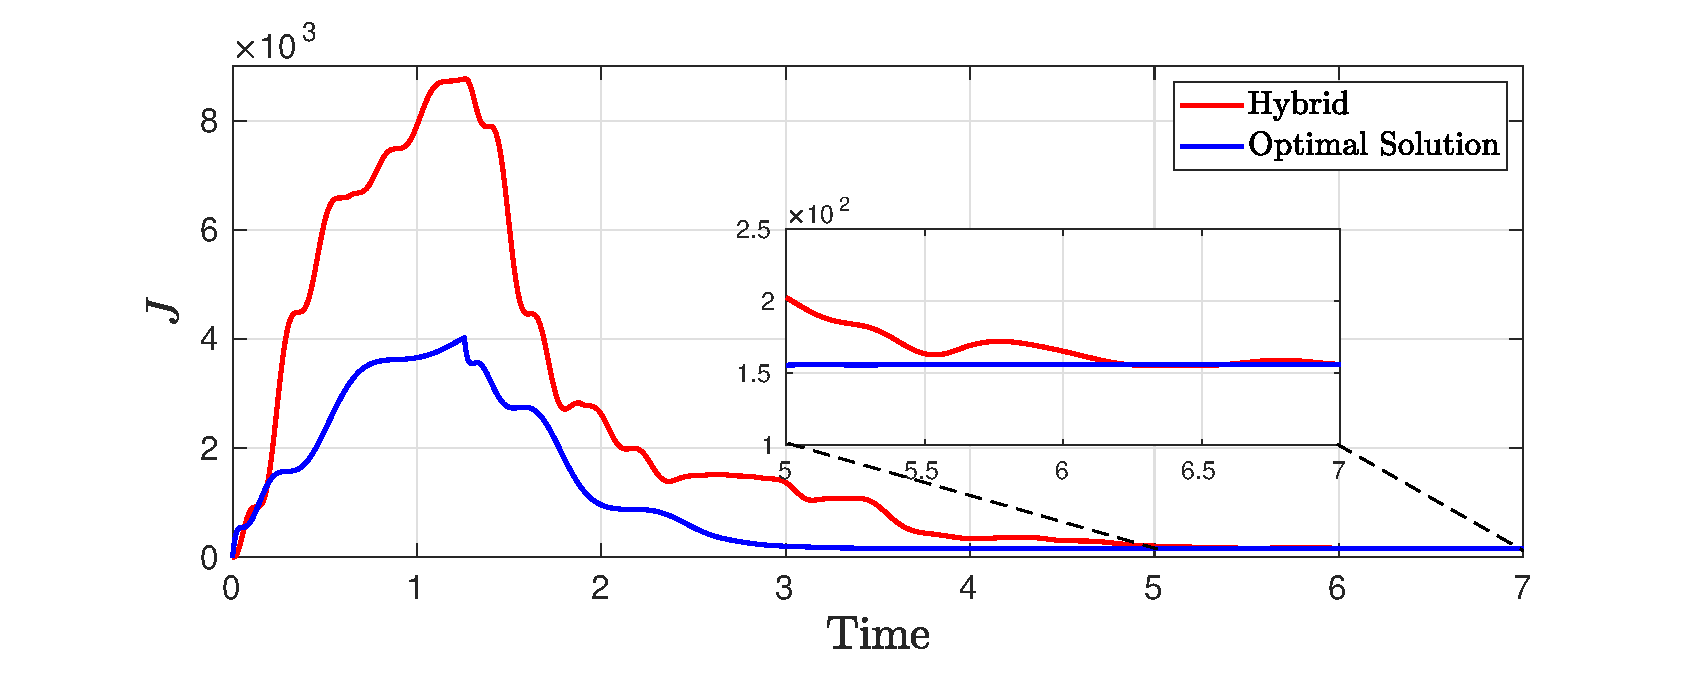
\includegraphics[width=\linewidth]{images/ch7/lqrall/sscosts}
    \caption{Cost in the presence of input allocation by means of a hybrid allocator (red), and of the periodic extension of the optimal solution to \Cref{prb:lqrall_optcont} (blue). The last value is the relevant one.}
    \label{fig:lqrall_sscosts}
  \end{figure}
  \begin{figure}[t]
    \centering
    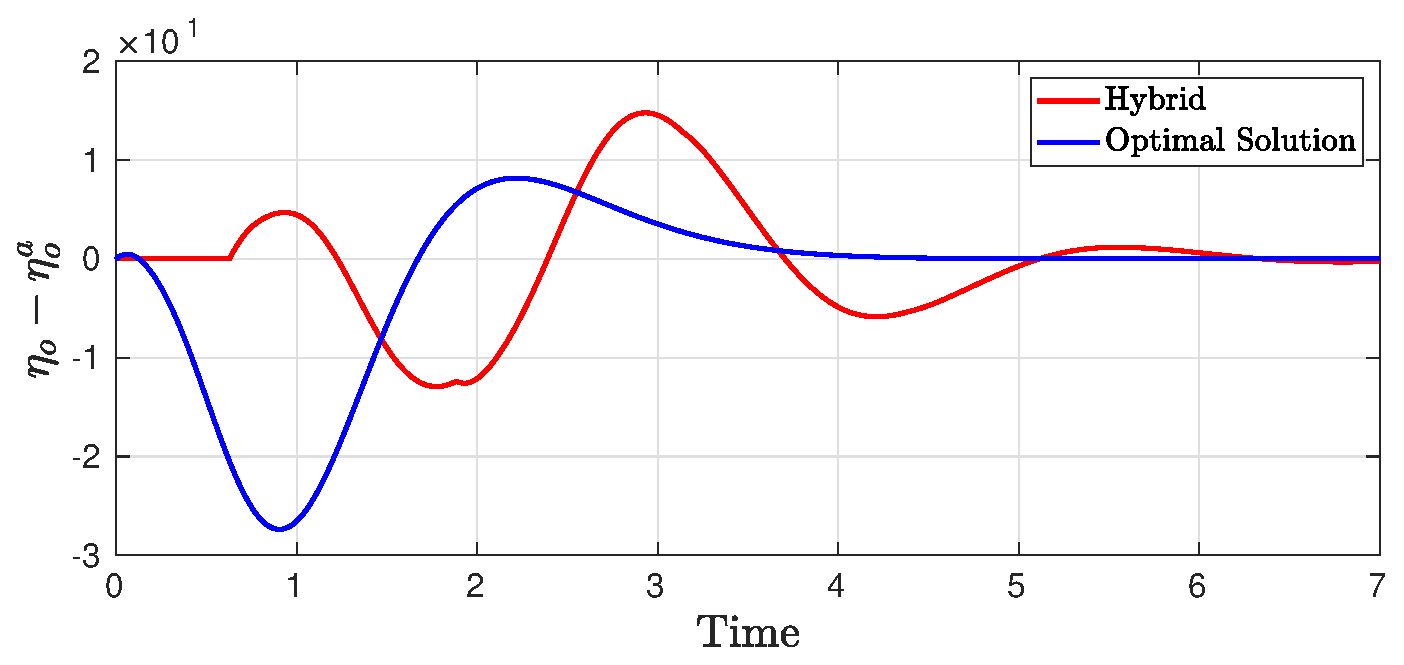
\includegraphics[width=.9\linewidth]{images/ch7/lqrall/ydiffs}
    \caption{Difference $\bbouto - \bboutoa$ between the regulated outputs of the closed loop in absence and presence of the allocator, respectively, for the hybrid allocator (red) and for the periodic extension of the optimal solution to \Cref{prb:lqrall_optcont} (blue).}
    \label{fig:lqrall_ydiffs}
  \end{figure}
  \begin{figure}[t]
    \centering
    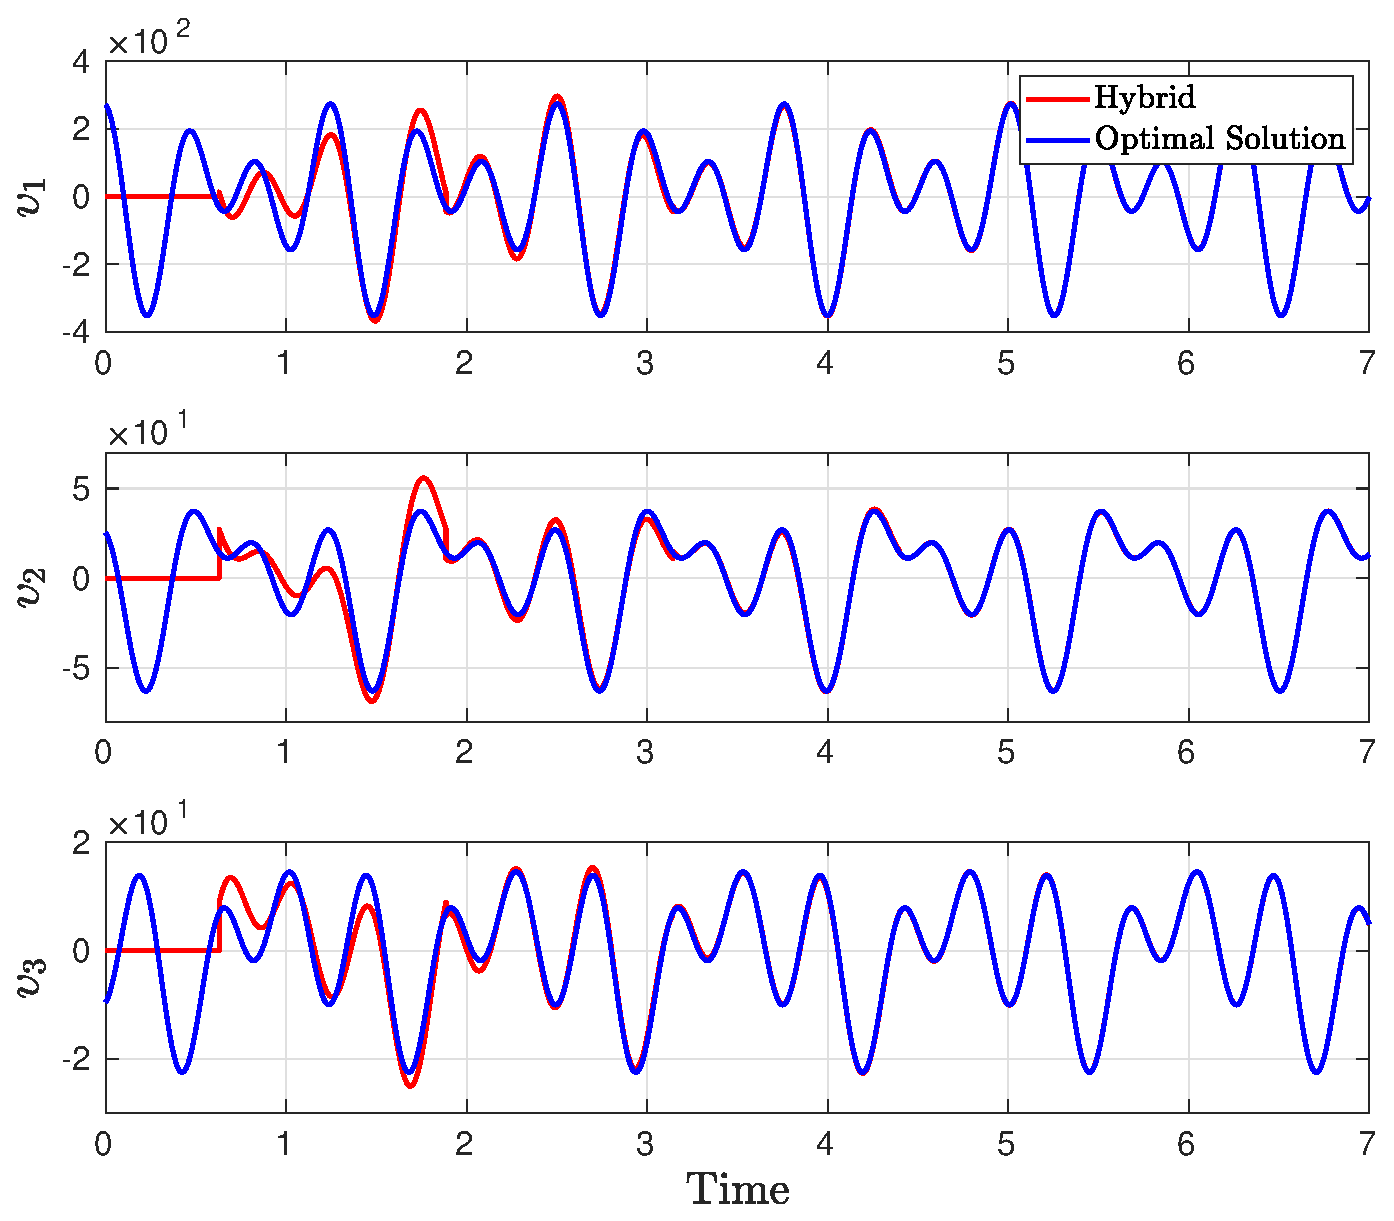
\includegraphics[width=.9\linewidth]{images/ch7/lqrall/ya}
    \caption{Outputs of a hybrid allocator (red) versus the components of the periodic extension of the optimal solution to \Cref{prb:lqrall_optcont} (blue).}
    \label{fig:lqrall_ya}
  \end{figure}

  The purpose of the proposed simulations is to compare the performance of a state-of-the-art hybrid allocator, designed as in \cite{galeani_dynamic_2014}, against the one that is implemented by applying the results presented above. The hybrid allocator is based on a gradient descent algorithm with the gradient decay rate $\gamma$ selected as $\gamma=2$. The implementation of the proposed allocator, based on the previous results, is based on the approach described in \Cref{rem:lqrall_apply}, namely applying a periodic extension of the optimal solution $v^{\star}$ to \Cref{prb:lqrall_optcont}. \Cref{fig:lqrall_sscosts} reports the time histories of the costs for the considered cases. After a transient motion, which is not relevant at all given that the cost has to be evaluated at steady-state, both solutions converge to the same value of the steady-state cost, which is the relevant one and is equal to $J(v^{\star})=155.836$. Even if, again, the transients in this plot are not relevant, it is interesting to note that the proposed solution converges must faster to the steady-state value, and also with a less intense transient, with respect to the state of the art. To evaluate the achieved output invisibility, consider the difference $\bbouto - \bboutoa$ between the regulated outputs of the closed loop in absence and presence of the allocator, respectively. The time histories of these differences for the proposed approach and the state of the art are depicted in \Cref{fig:lqrall_ydiffs}: the convergence to zero of both signals proves that both solutions, including the proposed one, meet the steady-state output invisibility requirement. The outputs of the state-of-the-art hybrid allocator are shown in \Cref{fig:lqrall_ya} against the components of $v^{\star}(t)$, showing that both signals become coincident after a transient phase.

  This study provides a first step towards the application of optimal control theory results within dynamic control allocation settings. The proposed approach allows the designer to build a control allocation device that acts, essentially, as a periodic function generator whose model is entirely determined in terms of its frequency components by \Cref{thm:lqrall_solution}. Conversely, the previous state-of-the-art solution is described by more complex hybrid dynamics.\closeexample
\end{example}
